%
\documentclass[12pt]{article}

% The usual packages
\usepackage{fullpage}
\usepackage{breakcites}
\usepackage{setspace}
\usepackage{endnotes}
\usepackage{float}
\usepackage{amsmath}
\usepackage{amsfonts}
\usepackage{amssymb}
\usepackage{rotating}
\usepackage{longtable}
\usepackage{microtype}
\usepackage{graphicx}
\usepackage{hyperref}
%\usepackage[usenames,dvipsnames]{color}
\usepackage{url}
\usepackage{natbib}
\usepackage{framed}
\usepackage{epigraph}
\usepackage{lipsum}
\usepackage[font=small,labelfont=sc]{caption}
\restylefloat{table}
\bibpunct{(}{)}{;}{a}{}{,}

% Set paragraph spacing the way I like
\parskip=0pt
\parindent=20pt

% Define mathematical results
\newtheorem{lemma}{Lemma}
\newtheorem{proposition}{Proposition}
\newtheorem{theorem}{Theorem}
\newtheorem{claim}{Claim}
\newenvironment{proof}[1][Proof]{\begin{trivlist}
\item[\hskip \labelsep {\bfseries #1}]}{\end{trivlist}}
\newenvironment{definition}[1][Definition]{\begin{trivlist}
\item[\hskip \labelsep {\bfseries #1}]}{\end{trivlist}}
\newenvironment{example}[1][Example]{\begin{trivlist}
\item[\hskip \labelsep {\bfseries #1}]}{\end{trivlist}}
\newenvironment{remark}[1][Remark]{\begin{trivlist}
\item[\hskip \labelsep {\bfseries #1}]}{\end{trivlist}}
\DeclareMathOperator*{\argmin}{arg\,min}
\DeclareMathOperator{\med}{med}


% Set up fonts the way I like
\usepackage{tgpagella}
\usepackage[T1]{fontenc}
\usepackage[bitstream-charter]{mathdesign}


%% Set up lists the way I like
% Redefine the first level
\renewcommand{\theenumi}{\arabic{enumi}.}
\renewcommand{\labelenumi}{\theenumi}
% Redefine the second level
\renewcommand{\theenumii}{\alph{enumii}.}
\renewcommand{\labelenumii}{\theenumii}
% Redefine the third level
\renewcommand{\theenumiii}{\roman{enumiii}.}
\renewcommand{\labelenumiii}{\theenumiii}
% Redefine the fourth level
\renewcommand{\theenumiv}{\Alph{enumiv}.}
\renewcommand{\labelenumiv}{\theenumiv}
% Eliminate spacing around lists
\usepackage{enumitem}
\setlist{nolistsep}

% Create footnote command so that my name
% has an asterisk rather than a one.
\long\def\symbolfootnote[#1]#2{\begingroup%
\def\thefootnote{\fnsymbol{footnote}}\footnote[#1]{#2}\endgroup}

% Create the colors I want
\usepackage{color}
\definecolor{darkred}{RGB}{100,0,0}

\hypersetup{
pdftitle={The Heavy Tails of Electoral Data}, % title
pdfauthor={Dan Baissa and Carlisle Rainey}, % author
pdfkeywords={robust linear regression} {outliers} {leverage}
pdfnewwindow=true, % links in new window
colorlinks=true, % false: boxed links; true: colored links
linkcolor=darkred, % color of internal links
citecolor=darkred, % color of links to bibliography
filecolor=darkred, % color of file links
urlcolor=darkred % color of external links
}

% enable comments in pdf
\newcommand{\kelly}[1]{\textcolor{blue}{#1}}
\newcommand{\carlisle}[1]{\textcolor{magenta}{#1}}


\begin{document}

\begin{center}
{\LARGE \textbf{The Heavy Tails of Electoral Data}}\\\vspace{2mm}
{ \textbf{The Importance of Robust Estimators}\symbolfootnote[1]{We thank Bill Clark and Matt Golder for making their data available to us. The analyses presented here were conducted with \texttt{R} 3.1.0. All data and computer code necessary for replication are available at \href{https://github.com/carlislerainey/heavy-tails}{
github.com/carlislerainey/meaningful-inferences}
.}}\\\vspace{2mm}


\vspace{10mm}

Dan Baissa\symbolfootnote[2]{Dan Baissa is an M.A. student in the Department of Political Science, University at Buffalo, SUNY, 520 Park Hall, Buffalo, NY 14260 (\href{mailto:dkbaissa@buffalo.edu}{
kellymcc@buffalo.edu}
).}

\vspace{3mm}

Carlisle Rainey\symbolfootnote[3]{Carlisle Rainey is Assistant Professor of Political Science, University at Buffalo, SUNY, 520 Park Hall, Buffalo, NY 14260 (\href{mailto:rcrainey@buffalo.edu}{
rcrainey@buffalo.edu}
).}
\end{center}

\vspace{10mm}

% Abstract
{\centerline{\textbf{Abstract}}}
\begin{quote}\noindent
Researchers studying the consequences of comparative electoral institutions, as well as other areas of political and social science, often estimate linear regression models on continuous outcomes of interest using least squares. These outcomes include measures of the number of political parties, proportionality, and vote share, among others. While it is well known that least-squares estimates are often sensitive to single, influential data point, this knowledge has not led to appropriate practices when using least-squares estimators. We highlight the important using more robust estimators (at least as a robustness check) and discuss several approaches to detect, summarize, and communicate the influence of particular data points. We conclude with a reanalysis of Clark and Golder (2006) an show that their conclusions depend on several influential data points. Removing these data or using a robust estimator substantially weaken their key conclusions about the conditional relationship between social heterogeneity and electoral rules in influencing the number of political parties.
 \end{quote}

% Add quote to first page
% \epigraph{}

%\begin{center}
%Manuscript word count: 
%\end{center}

% Remove page number from first page
\thispagestyle{empty}

% Start main text
\newpage
\doublespace

\section*{Introduction}

Our goal in this manuscript, our goals are to (1) highlight powerful, robust alternatives to least-squares estimators, (2) provide concrete, practical advice to substantive researchers using linear models, and (3) provide a compelling example that shows the importance of robust estimators.

\section*{Is a BLUE Estimator the ``Best'' Estimator?}

The linear regression model can be written as $E(y | X) = X\beta + \epsilon$, where $y$ is an outcome variable of interest (usually roughly continuous), $X$ is a $n \times (k + 1)$ matrix containing a single column of ones and $k$ columns holding $k$ explanatory variables, $\beta$ is a $(k + 1) \times 1$ matrix of model coefficients, and $\epsilon$ is an $n \times 1$ matrix of errors. Researchers in political science commonly estimate this model with ordinary least squares (OLS) by minimizing the squared residuals, $\hat{\beta}^{OLS} = \argmin S(b)$, where $S(b) = \sum_{i = 1}^n(y_i - X_ib)^2$. That is, OLS estimators choose the estimate $\hat{\beta}$ that minimizes the sum of the squared residuals. Under the assumption that the errors $\epsilon_i$ follow independent and identical normal distributions with mean zero and unknown variance, the OLS estimator is the minimum variance unbiased estimator (MVUE).

Even if the errors do not follow independent and identical normal distributions, the Gauss-Markov Theorem guarantees the least-squares estimator is the best (i.e., minimum variance) \textit{linear} unbiased estimator if the errors have mean zero and constant (and finite) variance. However, this should provide little comfort to researchers because their is little statistical or substantive reason to restrict themselves to \textit{linear} estimators.

At first glance, one might take the linearity restriction under Gauss-Markov to refer to the structure of the model, such that $E(y | X) = X\beta$ falls into the class of ``linear'' regression models, but  $E(y | X) = e^{X\beta}$ does not. Indeed, this is the sense in which we use ``linear'' in the term ``linear regression.'' However, the ``linear'' restriction in the Gauss-Markov Theorem refers to a highly technical and obscure statistical criterion that requires that the estimates be a linear function of the outcome variables, so that $\hat{\beta}_j = \lambda_1 y_1 + \lambda_2 y_2 + ... \lambda_n y_n$, so that the weights $\lambda_i$ are allowed to depend on $X$, but not on $y$.\footnote{Formally, linearity requires that $\hat{\beta} = My$, where $M$ depends on the matrix $X$. For the case of least-squares, $M = (X'X)^{-1}X'$.} In other words, Gauss-Markov does not require a linear \textit{model} of the form $E(y | X) = X\beta$, but it does require a linear estimator of the form $\hat{\beta}_j = \lambda_1 y_1 + \lambda_2 y_2 + ... \lambda_n y_n$. 

However, we argue that restricting ourselves to linear estimators is unnecessary and unproductive. There is no statistical reason to restrict ourselves to linear estimators, except for mathematical convenience, and there are substantive reasons to reject this restriction. For example, if the researcher is aware that one case has a unusually large outcome variable (conditional on the explanatory variables), then the researcher might wish to weight that case less than the other, more typical cases so that one atypical case does not exert several times more impact on the estimates than other, typical cases. Indeed, substantive researchers might wish to attach zero weight to extremely unusual cases because these cases might be due to a different substantive process.

It is not often appreciated that if the errors do not follow independent and identical normal distributions, then the OLS is no longer the MVUE--other estimators might outperform OLS.

Many researchers simply assume a statistical model for which a MVUE is easily available for little or no substantive reason. Knowing that the assumed model (e.g., normality) is \textit{in}orrect, these researchers are using this model as an approximation. But if the model is an approximation, then the desirable statistical properties are not longer guaranteed (e.g., MVUE). With this in mind, it makes more sense to use a robust estimator with the following qualitative properties:
\begin{enumerate}
\item Approximately unbiased in typical sample sizes for the assumed model and small, plausible deviations.
\item Excellent efficiency under the assumed model, though perhaps not the best possible efficiency.
\item Excellent efficiency under small deviations from the assumed model
\item Reasonable efficiency and bias in typical sample sizes with large deviations from the assumed model. 
\end{enumerate}

Mathematically, this suggests that applied researchers should not necessarily restrict themselves to unbiased estimators or minimum variance estimators under an assumed model. Instead, a more desirable criterion might be the mean squared error of the estimate under a wide range of deviations from the assumed model. The ``best'' model for a social scientist might not be the optimal estimator for an assumed model, but an estimable that works reasonably well for the assumed model and many substantively plausible deviations. 

To see the importance of this in practice, we simulated 10,000 data sets 50 observations of variables $x$ and $y$, where the relationship between $x$ and $y$ is given by $y = x + \epsilon$, where $\epsilon$ follows a $t$ distribution with three degrees of freedom. Note that the $t_3$ distribution is symmetric, bell-shaped, and resembles the normal distribution, except it has slightly heavier tails. For each of these 10,000 data sets we used least-squares to estimate the slope of the relationship between $x$ and $y$. Because we simulated these data, we know that the Gauss-Markov assumptions hold. This means that least-squares is the \textit{best} linear unbiased estimator. The left panel of Figure \ref{fig:lts-illustration} shows the distribution of the estimated slopes using least squares.

But consider a least trimmed squares (LTS) estimator in which we minimize the smallest 90\% of the residuals. This method literally throws away data. Though it lacks the elegant theory of the least-squares estimate, the right panel of Figure \ref{fig:lts-illustration} shows that it is essentially unbiased and, compared to the least-squares more efficient (standard deviation about 18\% smaller), and has a much smaller mean squared error (about 32\% smaller) . By any reasonable standard, it is a better estimator than the least squares estimator. This improvement is dropped by expanding our focus to non-linear estimators. In this case, the LTS estimator is not linear because it places zero weight on the largest 10\% of the residuals and weights of one on the smallest 90\% of the residuals.

\begin{figure}[H]
\begin{center}
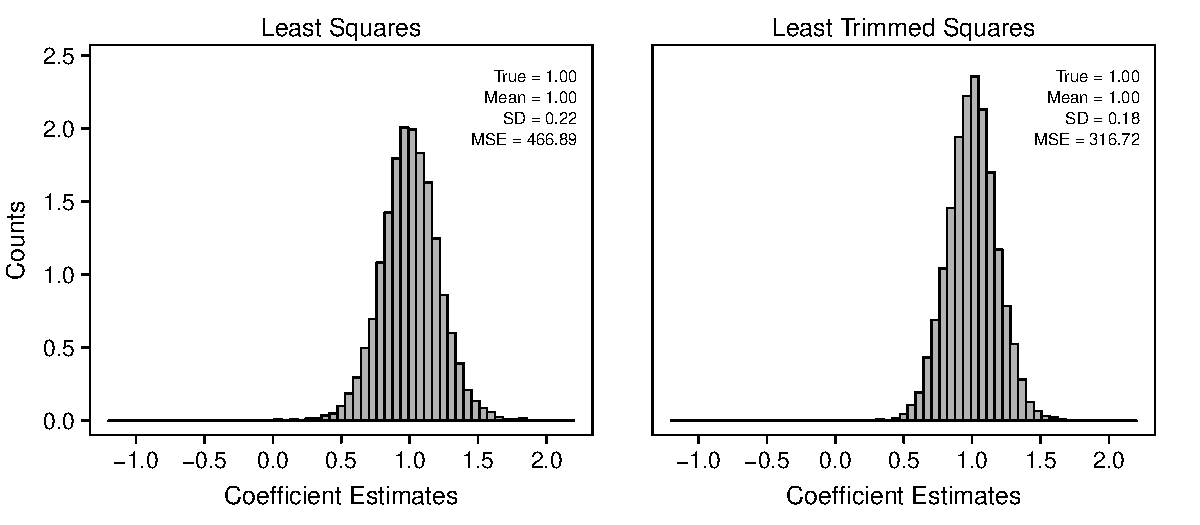
\includegraphics[scale = .7]{figs/lts-illustration.pdf}
\caption{caption here}\label{fig:lts-illustration}
\end{center}
\end{figure}

While the statistical properties of the least squares under the assumed normal-linear model are extremely well developed (e.g., MVUE), these properties are not nearly as well developed from robust alternatives. Some asymptotic results are available, but the closed-form theory is generally much weaker.

There has been a great deal of attention in the methodological literature to the sensitivity of standard errors to violations from the assumed model--and substantive scholars have paid attention. For example, White's (1980) seminal paper developing heteroskedasticity-consistent standard errors has received over 20,000 citations, making it one of the most cited papers in economics. Beck and Katz's (1995) introduction to panel corrected standard errors has received over 4,300 citations, making it one of the most cited political science papers ever.

On the other hand, there has been scant attention paid to the sensitivity of the estimates to similar violations. This is particularly problematic, since it makes little sense to find a good standard error for a poor estimate. Two papers in political science have addressed the issue of robust estimation. Western's (1995) introduces political scientists to robust estimators, but this work has been essentially ignored. The work is more broadly applicable than Beck and Katz (1995) and was published in the same year, but has received only 99 citations, or  about 2\% of the citations that Beck and Katz have received. Similarly, Demaris and Harden (2011) has received only one citation, and it comes from the authors themselves. Anderson's (2008) broad and accessible introduction to robust estimation methods has received only about 150 citations, most from outside political science.

This focus on obtaining reasonable standard errors at the expense of reasonable estimates can be seen in Gujarati (????, p. ??, ), a popular textbook for political science classes focusing on linear models. Though the text deals with robust standard errors in some detail, Gujarati writes (in a footnote):
\begin{quote}
In passing, note that the effects of departure from normality and related topics are often discussed under the topic of robust estimation in the literature, a topic \textit{beyond the scope of this book} [italics ours].
\end{quote}
Another popular textbook, Wooldridge (????) does briefly discuss robust estimators, though in a much more limited manner than his discussion of robust standard errors. Angrist and Pischke (2008), though, devote an entire chapter to robust standard errors and completely ignore robust estimation of model coefficients.

\section*{Dealing with Skewness: Transforming the Outcome}

Skewed error distribution create two problems for the linear model. First, because least squares models the quantity $E(Y | X)$ and the mean is not a good summary of location for skewed variables. Symmetric error distributions are easier to understand. Second, and perhaps most importantly, we take skewed error distributions as a lack of model fit. For example, it is theoretically intuitive to believe that the explanatory variables should have increasing effects non-negative outcome variables, such as an individual's annual income. For example, rather than a college degree increasing one expected income by \$10,000, perhaps it increases one's expected income by 10\%. We consider skewed error distributions as evidence that the basic structure of the model could be improved.

Points that are unusual prior to transformation might be quite typical after transformation.

Even if we remain indifferent toward the theoretical implications of skewed error distributions, we must remain cautious about the statistical implications. The performance of least squares estimators improves as the error distribution approaches a normal distribution. Further, the theoretical properties of alternative, more robust estimators, such as the $M$-estimator we discuss below, depend on a symmetric error distribution distribution.

It is quite common in disciplines such as economics, for example, to log-transform non-negative outcome variables by default. The motivation is that since non-negative (or strictly positive) outcomes are bounded below by zero, then these variables are likely skewed to the right. In this case, the model $\log(y) = X\beta + \epsilon$ will likely provide a better approximation to the data.

While we agree with the spirit of this suggestion, we have much more precise empirical methods for choosing \textit{whether} and \textit{how} to transform the outcome variable $y$. Box and Cox (1964) proposed the Box-Cox transformation 

\begin{displaymath}
   y^{(\lambda)} = BC(y, \lambda) = \left\{
     \begin{array}{lr}
       \dfrac{y^\lambda - 1}{\lambda} & \text{for } \lambda \neq 0\\
       \log y & \text{for } \lambda \neq 0
     \end{array}
   \right.
\end{displaymath}.

\noindent In this case, the model becomes $y^{(\lambda)} = X\beta + \epsilon$. The researcher can easily use maximum likelihood to obtain estimates $\hat{\lambda}$ and standard errors for the transformation parameter $\lambda$. This is particularly convenient because if $\hat{\lambda}$ is near one, this suggests no transformation is needed and if $\hat{\lambda}$ is near zero, then only an intuitive log-transformation is needed.

It is quite easy to assess the skewness in the residuals using a simple histogram of the residuals or a QQ plot of the residuals compared to their normal quantiles. For a formal test of skewness, one might use a direct test for symmetry on residuals $\hat{e}$, such as the Mira test (Mira 1999) or simply test whether $\lambda \neq 1$ under the Box-Cox framework. However, the important point is not to argue for any particular test, but to point out (1) that asymmetries worsen the performance of least squares and alternative methods and (2) this potential problem can and should be addressed using simple transformations that are easy to implement.

However, applying transformation to the outcome variable $y$ does raise an interpretational difficulty. The usual, untransformed linear model is given by $y = X\beta + \epsilon$ and the quantity of interest is $E(y | X)$ or $\frac{\partial E(y | X)}{\partial x_j}$. For concreteness, consider the log-transformation. Using the same logic, then the model is $log(y) = X\beta + \epsilon$ and we might take the quantity of interest to be $E[\log(y) | X]$ or $\frac{\partial E[\log(y) | X]}{\partial x_j}$. However, these quantities are not as easy to understand substantively--$\frac{\partial E[\log(y) | X]}{\partial x_j}$ is more difficult to understand than $\frac{\partial E(y | X)}{\partial x_j}$. To make the results more understandable, we simply need to ``undo'' the transformation. However, it is important to note that $E[\log(y) | X] \neq \log [E(y | X)]$, which means that the log cannot simply be undone (without additional computation) because $e^{E[\log(y) | X]} \neq E(y | X)$. 

However, in the context of skewed distributions, the mean $E(\dot)$ might be a misleading summary of the ``center'' of the data. While the mean is often more mathematically convenient, the median offers a better summary of location than the mean. Further, the median has an intuitive interpretation because there is a one-half of the distribution lies above the median and one-half lies below. This mean that there is approximately a one-half chance that $y |X$ falls above $\med(y | X)$ and a one-half changes that $y |X$ falls below.

In addition to the intuitive substantive interpretation of $\med(y | X)$, the median has another desirable property. Because the log-transformation is order-preserving $\med[\log(y) | X] = \log [\med(y | X)]$, which means that the log \textit{can} easily be undone because $e^{med[\log(y) | X]} = e^{\log[\med(y | X)]} = \med(y | X)$. Therefore, by adopting $\med(y | X)$ and $\frac{\partial \med(y | X)}{\partial x_j}$, one gains a more intuitive quantity of interest and can easily move between transformed and untransformed outcomes (e.g., $\med[\log(y)] \rightarrow \med(y)$). This holds for the more general case of $y^{(\lambda)}$ in addition to $\log(y)$.

To obtain quantities of interest for $\med(y)$ when the estimated model has the generic form $y^{(\lambda)} = X\beta + \epsilon$, one can simply use the algorithm described in King, Tomz, and Wittenberg (2000).
\begin{enumerate}
\item Estimate the model $y = X\beta + \epsilon$ using least squares to obtain the estimated model coefficients $\hat{\beta}^{ls}$ and residuals $\hat{e}^{ls}$. Evaluate whether the assumption of the normal errors matches the estimated residuals using histograms and QQ plots.
\item If needed, estimate the Box-Cox transformation parameter $\hat{\lambda}$ using maximum likelihood. (If the values one or zero fall within the confidence interval, then one may wish to use those values to maintain the direct interpretability of the model coefficients.)
\item Estimate the transformed model $y^{(\lambda)} = X\beta + \epsilon$ using least squares to obtain the estimated model coefficients $\hat{\beta}^{ls}_{trans}$, residuals $\hat{e}^{ls}_{trans}$, and covariance matrix $\Sigma^{ls}_{trans}$.
\item Choose a hypothetical case or set of cases $X_{pred}$ for which to calculate the quantity of interest. If one is interested in calculating a first difference, it is convenient to use $X_{hi}$ and $X_{lo}$, where the first-difference $\Delta(y, X_{hi}, X_{lo}) = \med(y | X_{hi}) - \med(y | X_{lo})$.
\item Following King, Tomz, and Wittenberg (2000), for $i$ from one to a large (e.g., 1,000) number of iterations $n_{sims}$:
	\begin{enumerate}
	\item Simulate $\tilde{\beta}^{ls}_{trans} \sim N\left(\hat{\beta}^{ls}_{trans}, \Sigma^{ls}_{trans}\right)$.
	\item Calculate and store $\tilde{Q}_i = \med(y | X_{red}, \tilde{\beta}^{ls}_{trans}) = X_{red}\tilde{\beta}^{ls}_{trans}$ or, if interested in the first-difference, $\tilde{Q}_i = \tilde{\Delta}(y, X_{hi}, X_{lo}, \tilde{\beta}^{ls}_{trans}) = X_{hi}\tilde{\beta}^{ls}_{trans} - X_{lo}\tilde{\beta}^{ls}_{trans}$.
	\end{enumerate}
\item Summarize the $n_{sims}$ simulations. The mean or median of $\tilde{Q}_i$ serves as an estimate of $\med(y | X_{pred})$, the standard deviation of $\tilde{Q}_i$ serves as an estimate of the standard error of $\med(y | X_{pred})$, and the 5th and 95th percentiles of $\tilde{Q}_i$ serve as an estimate of the (likely asymmetric) 90\% confidence interval for $\med(y | X_{pred})$.
\end{enumerate}

\section*{Dealing with Heavy-Tails: $M$-Estimation}

In spite of the scant attention paid to robust estimators in political science, statisticians have developed and refined many robust methods since the seminal work of Box (1953) and Huber (1964). Huber and Ronchetti (2009) provide a detailed review of these developments and Anderson (2008) provides an accessible introduction. 

Adjudicating among these many robust alternatives to least squares is beyond the scope of our paper, but, to fix ideas, we do introduce one robust estimator in detail which has several desirable properties--the $M$-estimator with Tukey's biweight function. 

While least squares yields the coefficients that minimize the sum of the squared residuals, so that $\hat{\beta}^{ls} =\argmin_{b} \sum_{i = 1}^n (y_i - X_ib)^2$, M-estimation minimizes an arbitrary, less-rapidly increasing function of the residuals $\hat{\beta}^{\rho} =\argmin_{b} \sum_{i = 1}^n \rho(y_i - X_ib)$. For example, Harden and Desmarais (2011) recommend the least absolute deviation (LAD) estimator that chooses $\rho(\dot) = abs(\dot)$. However, other estimators offer similarly robust alternatives. In particular, we recommend Tukey's biweight function, so that

\begin{displaymath}
   \rho_{bw}(r_i) = \left\{
     \begin{array}{lr}
       \dfrac{k^2}{6}\left\{ 1 - \left[ 1 - \left( \dfrac{r_i}{k} \right)^2 \right]^3\right\} & \text{for } |r_i| \leq k\\
	\dfrac{k^2}{6} & \text{for } |r_i| > k 
\end{array}
   \right.,
\end{displaymath}.

where $r_i = y_i - X_ib$.

[Discuss the desirable substantive properties of bw, such as fitting the majority of the data well and ignoring, rather than simply down weighting unusual data.]

Two cautions are in order. Second, the optimization problem is not convex, so standard optimization routines can produce a local rather than a global minimum. Second, because the solution is not scale invariant, the residuals $\hat{e_i}$ are standardized by a robust estimate of scale $\hat{\sigma}_{(mad)}$, which must of course be estimated jointly, so that $\hat{\beta}^{bw} =\argmin_{b} \sum_{i = 1}^n \rho_{bw}\left(\dfrac{y_i - X_ib}{\hat{\sigma}_{mad}}\right)$, where $\hat{\sigma}_{mad} = \dfrac{\med\left( |y - X\b|\right)}{0.6745}$. Dividing by 0.6745 makes $\hat{\sigma}_{mad}$ a consistent estimator of the standard deviation of normal errors.

The model parameters $\hat{\beta}^{bw}$ and $\hat{\sigma}_{bw}$ can be quickly estimated jointly using the following iterative algorithm.
\begin{enumerate}
\item Start with initial estimate of the coefficients $\hat{\beta}^{(0)}$. The choice of initial estimator is not trivial. In the case of extreme outliers and/or many parameters, starting with least squares might lead the algorithm to a local minimum. We recommend the least trimmed squares method discussed earlier to obtain starting values.
\item Extract the residuals $r^{(0)} = X\hat{\beta}^{(0)}$. Use these residuals to estimate the rescaled MAD so that $\hat{\sigma}^{(0)}_{mad} = \dfrac{\med\left( |y - X\hat{\beta}^{(0)}|\right)}{0.6745}$.
\item ssign weights $w$ according to the function $\rho$ and denote $\text{diag}(w) = W$.
\item For $i$ from one until convergence:
	\begin{enumerate}
	\item Using $\hat{\beta}^{(i-1)}$ and $\hat{\sigma}^{(i-1)}_{mad}$ assign weights $w$ according to the function $\rho$ and denote $\text{diag}(w) = W$.
	\item Calculate $\hat{\beta}^{(i)} = (X'WX)^{-1}X'Wy$.
	\item Calculate $\hat{\sigma}^{(i)}_{mad} = \dfrac{\med\left( |y - X\hat{\beta}^{(0)}|\right)}{0.6745}$
	\item The algorithm has converged when $r^{(i-1)} \approx r^{(i)}$.
	\end{enumerate}
\end{enumerate}

[Discuss some asymptotic properties of M-estimators]

[Discuss standard errors for m-estimators.]

[Simulations comparing LS, LAD, and BW]

Too get a sense of how close a $t_{10}$ distribution is to a normal distribution, note that a Shapiro-Wilk test only successful rejects the null in about 65\% of repeated samples if 500 observation are simulated from a $t_{10}$ distribution.\footnote{One needs about 750 samples to reach 80\% power.} It is essentially impossible to spot the differences between the normal and $t_{10}$ density functions without plotting the two directly on top of each other, in which case the $t_{10}$ has \textit{slightly} heavier tails.

\begin{figure}[h!]
\begin{center}
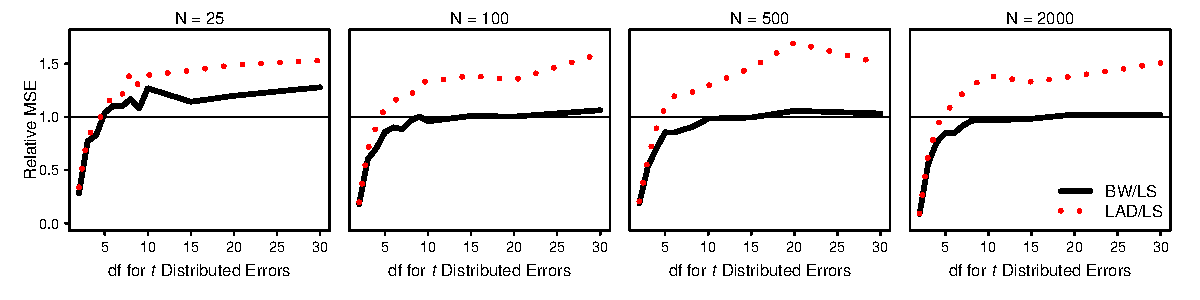
\includegraphics[width = \textwidth]{figs/mc-sims.pdf}
\caption{caption here}\label{fig:mc-sims}
\end{center}
\end{figure}

\begin{table}
{\tiny
% quantreg::latex.table(x = ta, file = "doc/tabs/mc-sims-100",      rowlabel = "", cgroup = c("Mean", "Standard Deviation", "Mean Squared Error"),      rgroup = c("Absolute Performance", "Relative Performance"),      n.rgroup = c(3, 2), dec = 3, table.env = FALSE, label = "tab:mc-sims-100") 
%
\begin{center}
\begin{tabular}{|l||c|c|c|c||c|c|c|c||c|c|c|c|} \hline
\multicolumn{1}{|l||}{\bf }&\multicolumn{4}{c||}{\bf Mean}&\multicolumn{4}{c||}{\bf Standard Deviation}&\multicolumn{4}{c|}{\bf Mean Squared Error}\\ \cline{2-13}
\multicolumn{1}{|l||}{}&\multicolumn{1}{c|}{Lapl.}&\multicolumn{1}{c|}{$t_2$}&\multicolumn{1}{c|}{$t_{10}$}&\multicolumn{1}{c||}{Norm.}&\multicolumn{1}{c|}{Lapl.}&\multicolumn{1}{c|}{$t_2$}&\multicolumn{1}{c|}{$t_{10}$}&\multicolumn{1}{c||}{Norm.}&\multicolumn{1}{c|}{Lapl.}&\multicolumn{1}{c|}{$t_2$}&\multicolumn{1}{c|}{$t_{10}$}&\multicolumn{1}{c|}{Norm.}\\ \hline
{\bf Absolute Performance}&&&&&&&&&&&&\\
~~Least Squares&~~~0.999&~~~1.000&~~~1.001&~~~0.999&~~~0.151&~~~0.319&~~~0.114&~~~0.099&~227.419&1016.182&~130.867&~~98.850\\ 
~~Least Absolute Deviation&~~~0.999&~~~0.999&~~~1.003&~~~1.000&~~~0.126&~~~0.146&~~~0.131&~~~0.124&~159.499&~212.360&~172.911&~154.714\\ 
~~Tukey's Biweight&~~~1.000&~~~0.999&~~~1.001&~~~0.999&~~~0.131&~~~0.138&~~~0.113&~~~0.102&~172.043&~189.519&~127.731&~104.759\\ \hline
{\bf Relative Performance}&&&&&&&&&&&&\\
~~LAD/LS&~~~1.001&~~~0.999&~~~1.002&~~~1.001&~~~0.837&~~~0.457&~~~1.149&~~~1.251&~~~0.701&~~~0.209&~~~1.321&~~~1.565\\ 
~~BW/LS&~~~1.001&~~~1.000&~~~1.000&~~~1.000&~~~0.870&~~~0.432&~~~0.988&~~~1.029&~~~0.757&~~~0.187&~~~0.976&~~~1.060\\ 
\hline
\end{tabular}
\end{center}

}
\caption{Summarizes of the Monte Carlo simulations for four different error distributions. The true statistical model is $y_i = \beta_0 + \beta_1x_1 + \beta_2 x_2 + \beta_3 x_3 + \epsilon_i$, where $\beta_0 = 0$ and $\beta_1 = \beta_2 = \beta_3 = 1$ with sample size 100 and $x_i$ following and approximately normal distribution. All the estimators are essentially unbiased for these symmetric error distributions. However, the efficiency varies across distributions. The Laplace and $t_2$ distributions have very heavy tails. The $t_10$ distribution has \textit{slightly} heavier tails than the normal distribution (barely detectable, even when plotted on top of each other). The normal distribution is typically assumed by the least squares model. Notice that the LAD and the BW estimators perform much better than LS for the heavy-tailed Laplace and $t_2$ distributions. However, the performance of the LAD estimator is much worse for the lighter-tailed $t_10$ and Normal distributions. The biweight estimator, on the other hand, performs almost as well as the normal for these distributions.}\label{tab:mc-sims-100}
\end{table}

\begin{table}
{\tiny
% quantreg::latex.table(x = ta, file = "doc/tabs/mc-sims-100",      rowlabel = "", cgroup = c("Mean", "Standard Deviation", "Mean Squared Error"),      rgroup = c("Absolute Performance", "Relative Performance"),      n.rgroup = c(3, 2), dec = 3, table.env = FALSE, label = "tab:mc-sims-100") 
%
\begin{center}
\begin{tabular}{|l||c|c|c|c||c|c|c|c||c|c|c|c|} \hline
\multicolumn{1}{|l||}{\bf }&\multicolumn{4}{c||}{\bf Mean}&\multicolumn{4}{c||}{\bf Standard Deviation}&\multicolumn{4}{c|}{\bf Mean Squared Error}\\ \cline{2-13}
\multicolumn{1}{|l||}{}&\multicolumn{1}{c|}{Lapl.}&\multicolumn{1}{c|}{$t_2$}&\multicolumn{1}{c|}{$t_{10}$}&\multicolumn{1}{c||}{Norm.}&\multicolumn{1}{c|}{Lapl.}&\multicolumn{1}{c|}{$t_2$}&\multicolumn{1}{c|}{$t_{10}$}&\multicolumn{1}{c||}{Norm.}&\multicolumn{1}{c|}{Lapl.}&\multicolumn{1}{c|}{$t_2$}&\multicolumn{1}{c|}{$t_{10}$}&\multicolumn{1}{c|}{Norm.}\\ \hline
{\bf Absolute Performance}&&&&&&&&&&&&\\
~~Least Squares&~~~0.999&~~~1.000&~~~1.001&~~~0.999&~~~0.151&~~~0.319&~~~0.114&~~~0.099&~227.419&1016.182&~130.867&~~98.850\\ 
~~Least Absolute Deviation&~~~0.999&~~~0.999&~~~1.003&~~~1.000&~~~0.126&~~~0.146&~~~0.131&~~~0.124&~159.499&~212.360&~172.911&~154.714\\ 
~~Tukey's Biweight&~~~1.000&~~~0.999&~~~1.001&~~~0.999&~~~0.131&~~~0.138&~~~0.113&~~~0.102&~172.043&~189.519&~127.731&~104.759\\ \hline
{\bf Relative Performance}&&&&&&&&&&&&\\
~~LAD/LS&~~~1.001&~~~0.999&~~~1.002&~~~1.001&~~~0.837&~~~0.457&~~~1.149&~~~1.251&~~~0.701&~~~0.209&~~~1.321&~~~1.565\\ 
~~BW/LS&~~~1.001&~~~1.000&~~~1.000&~~~1.000&~~~0.870&~~~0.432&~~~0.988&~~~1.029&~~~0.757&~~~0.187&~~~0.976&~~~1.060\\ 
\hline
\end{tabular}
\end{center}

}
\caption{Summary of Monte Carlo simulations identical to those in Table Table \ref{tab:mc-sims-100}, except with the sample size as 1,000 rather than 100. The basic conclusion remains unchanged. The biweight estimator works well for heavy-tailed distributions and nearly as well as least squares for the normal distribution.}\label{tab:mc-sims-1000}
\end{table}



\singlespace
\bibliographystyle{apsr_fs}
%\bibliography{/Users/carlislerainey/Dropbox/papers/bibliography/bibliography.bib}
\bibliography{/Users/rcrainey/Dropbox/papers/bibliography/bibliography.bib}


\section*{Replication of Clark and Golder (2006)}

\begin{figure}[H]
\begin{center}
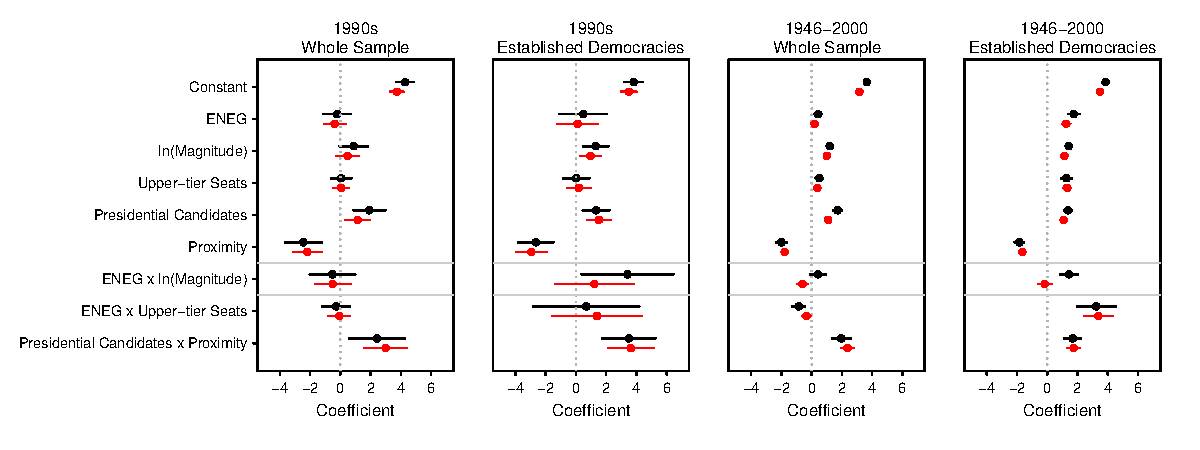
\includegraphics[scale = .8]{figs/cg-coef-plots.pdf}
\caption{Replication of Clark and Golder (2006) using MM-estimation with explanatory variables standardized to have mean zero and standard deviation one-half. The black lines and points show the OLS estimates and 90\% confidence intervals and the red lines and points show the MM estimates and confidence intervals. Notice that the coefficient for the product of the effective number of ethnic groups and the district magnitude changes drastically with the choice of estimator.}\label{fig:cg-coef-plots}
\end{center}
\end{figure}

\begin{figure}
%\centering
\begin{minipage}[t]{0.48\textwidth}
%\centering
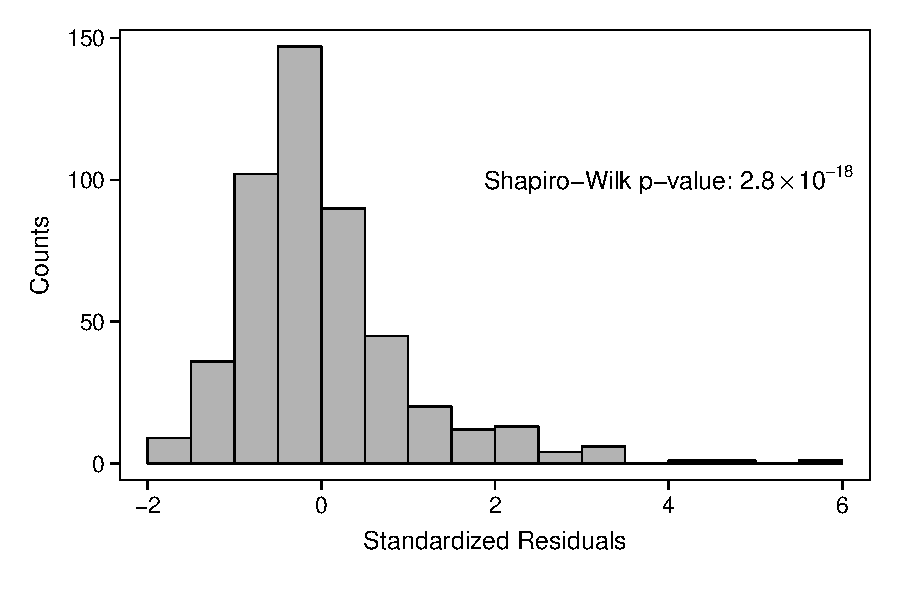
\includegraphics[width = \textwidth]{figs/cg-residuals-hist.pdf}
\caption{A histogram showing the distribution of the residuals from Clark and Golder's (2006) main model. Notice that these residuals do not seem approximately normal. They have a strong skew and heavy tail to the right. For example, one would rarely expect to observe residuals more that three standard deviations from zero if the assumption of normality holds. In these data, we have several residuals more that three standard deviations away and one nearly six standard deviations away. This suggests that some transformation of the outcome variable might be useful.}
\end{minipage}\hfill
\begin{minipage}[t]{0.48\textwidth}
%\centering
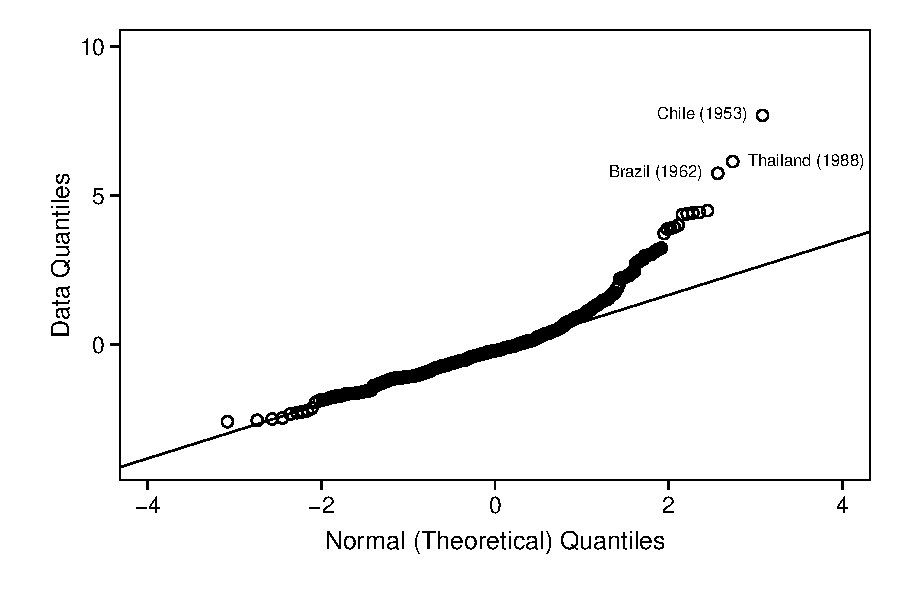
\includegraphics[width = \textwidth]{figs/cg-qq-plot.pdf}
\caption{A QQ plot showing the deviation of the residuals from normality. If the residuals were approximately normal, then the points in the QQ plot would approximately follow the line. However, notice that the positive residuals deviate sharply from the theoretical expectations. This also suggests that some transformation of the outcome variable might be useful.}
\end{minipage}
\end{figure}

\begin{figure}[h!]
\begin{center}
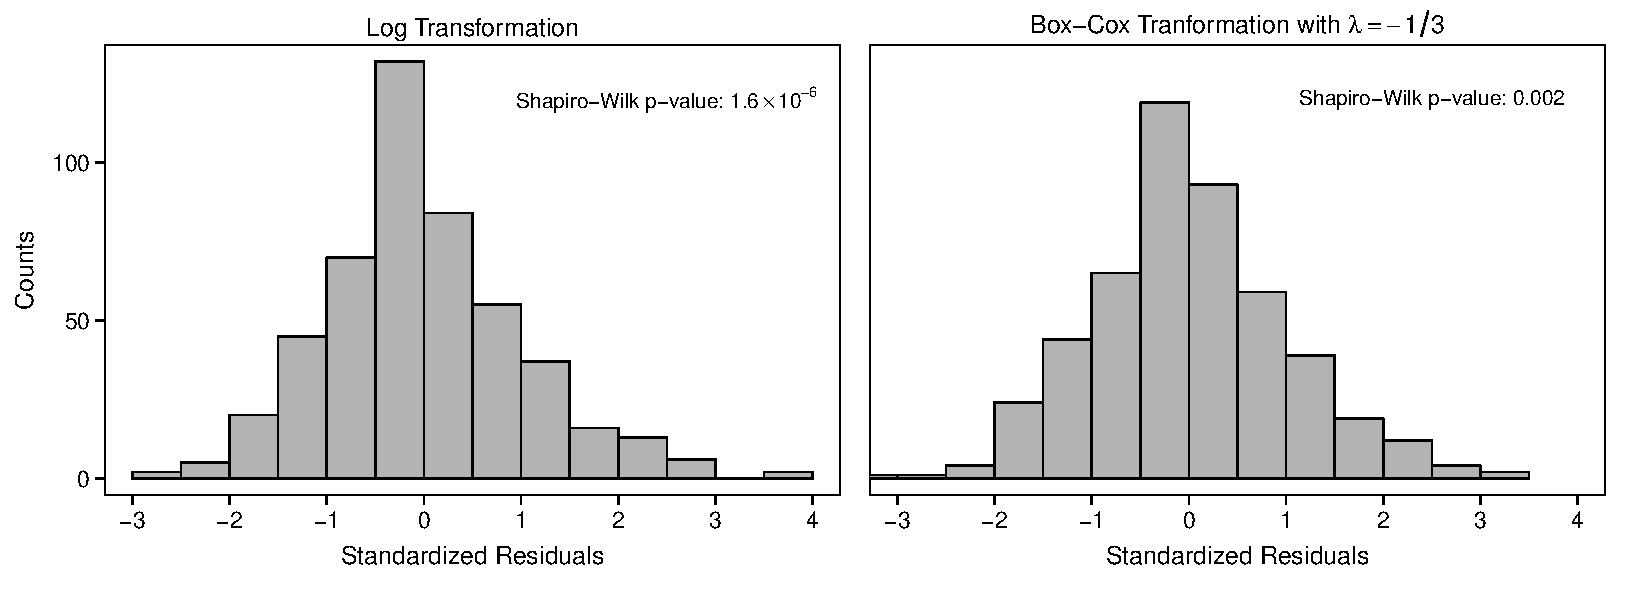
\includegraphics[width = \textwidth]{figs/cg-trans-residuals-hist.pdf}
\caption{}\label{fig:cg-trans-residuals-hist}
\end{center}
\end{figure}

But what to we learn from carefully considering whether the residuals match the assumptions of the normal linear model?
\begin{itemize}
\item \textit{Perhaps Duverger's logic is not as well-supported empirically as the literature would suggest.} Indeed, the evidence offered by the normal linear model seems to hinge on a few cases that seem inconsistent with the majority of the data. However, rejection of Duverger's theory or Clark and Golder's (2006) analysis is premature for three reasons. First, the theoretical logic for Duverger's hypotheses is clear and compelling (CITES). Second, many studies beyond Clark and Golder (2006), including experimental work, find substantial empirical support for the hypotheses. Finally, the biweight $M$-estimator suggests several potential shortcomings in terms of theory and measures that might currently undermine the evidence for these theories.
\item \textit{Room for improvement exists in the measurement of ``established democracies.''}
\item \textit{Room for improvement exists in the measurement of ``social heterogeneity.''}
\item \textit{We need a stronger theory about the dynamics with which systems reach an equilibrium number of parties.}
\item \textit{We need additional research into how systems respond to the introduction of additional parties into formerly authoritarian, single-party systems.}
\end{itemize}

\newpage
\doublespace
\begin{appendix}
\begin{center}
\textbf{{\LARGE Appendix}}\\\vspace{2mm}
\textbf{{\large The Heavy Tails of Electoral Data}}\\\vspace{2mm}

\end{center}
\section{}


\end{appendix}


\end{document}